\documentclass[11pt]{article}
\usepackage[margin=2.5cm]{geometry}
\usepackage[T1]{fontenc}
\usepackage[utf8]{inputenc}
\usepackage{lmodern}
\usepackage{amsmath}
\usepackage{siunitx}
\usepackage{graphicx}
\usepackage{booktabs}
\usepackage[numbers,sort&compress]{natbib}
\usepackage[hidelinks]{hyperref}
\usepackage{caption}
\captionsetup{font=small,labelfont=bf}
\graphicspath{{figures/}{../figures/mesh/}}
\sisetup{group-separator={\,},group-minimum-digits=4}

\title{Tonal noise of a ducted desk fan with serrated blades:\\
sliding-mesh URANS, Ffowcs Williams--Hawkings prediction,\\
and a force-based verification of the acoustic output}
\author{Cl\'ement Dumeril\thanks{University of California, Berkeley (MEng). Work carried out in May--June 2026 at
Polytechnia, an engineering consultancy co-founded by the author; re-analysis of the acoustic data in October 2026.
Repository: \url{https://github.com/clementdumeril/ducted-fan-aeroacoustics}.}}
\date{October 2026}

\begin{document}
\maketitle

\begin{abstract}
A computational-aeroacoustics chain was set up for a five-blade ducted desk fan with owl-inspired serrated
trailing edges. The incompressible flow is solved with OpenFOAM (URANS, $k$--$\omega$ SST) on a
\num{1.95}-million-cell mesh with a cyclicAMI rotor zone at \SI{1509}{rpm}, and the Farassat 1A form of the
Ffowcs Williams--Hawkings (FW-H) equation gives the pressure at four microphones \SI{1}{m} away. The rotor
produces \SI{43.3}{mN} of thrust and \SI{108}{m^3/h}. The spectra contain the blade-passing frequency (BPF,
\SI{126}{Hz}) 20 to \SI{28}{dB} above the local floor, a once-per-revolution tone confined to the rotor plane whose
directivity matches the rotating in-plane force found in the blade loads, and a comb of lines spaced
\SI{100.5}{Hz} above \SI{600}{Hz} that follows periodic bursts in the blade force. A verification of the FW-H output
against compact-dipole estimates built from the integrated pressure force reproduces the directivities but not the
amplitudes ($-9$, $+14$ and $-18$~dB for the mean load, the \SI{25}{Hz} tone and the BPF), which points to an input
or scaling problem in the acoustic step. The results are therefore the tone frequencies and directivities, not the
levels. No mesh or time-step independence study was run, and the effect of the serrations is not measured.
\end{abstract}

\section{Introduction}

The tonal noise of a low-speed fan is radiated by the unsteady force the blades exert on the air. A rotor of $Z$
identical blades turning at $n$ revolutions per second radiates at the blade-passing frequency $Zn$ and its
harmonics \citep{lowson1965}; interaction with $V$ stationary struts adds circumferential modes $m=kZ-sV$
\citep{tyler1962}, and any asymmetry between blades adds tones at multiples of $n$. Trailing-edge serrations,
inspired by owl feathers, act mainly on broadband noise by reducing the scattering of boundary-layer turbulence at
the edge \citep{howe1991,lyu2016}. A recent study combined owl-feather serrations with cicada-wing geometry on small
propellers and reported lower overall levels and higher propulsive efficiency \citep{wei2024}; it was the starting
point of the fan studied here.

The question was practical: can an open-source chain, run on a small self-built cluster, give a usable acoustic
signature of a 3D-printable desk fan before it is built, and which parts of that signature can be trusted? The fan
has five serrated blades in a short duct, with a motor hub held by three arms. The contributions are:
\begin{itemize}
  \item a sliding-mesh URANS and FW-H set-up for the fan (OpenFOAM, libAcoustics) that runs stably;
  \item a per-record spectral analysis of the FW-H signals that identifies the BPF and its harmonics, a
    once-per-revolution tone explained by the force history, and a high-frequency line comb tied to periodic bursts
    in the blade force;
  \item a verification of the FW-H amplitudes against compact-dipole estimates built from the integrated blade
    pressure force, which separates the reliable part of the acoustic output (frequencies, directivities) from the
    unreliable part (levels).
\end{itemize}

\section{Related work}

The Ffowcs Williams--Hawkings equation \citep{ffowcswilliams1969} extends Lighthill's analogy to sources on moving
surfaces. For surfaces moving at subsonic speed, Farassat's Formulation 1A gives the thickness and loading noise as
retarded-time surface integrals with the observer-time derivative taken analytically \citep{farassat2007}; it is
the standard tool for rotor tonal noise \citep{brentner2003}. \citet{tao2026}, in a preprint, argue that
Formulation 1A omits a term linked to the variation of the surface normal. The field of a point force in motion,
which underlies the compact-dipole estimates of Section~\ref{sec:verif}, was derived by \citet{lowson1965}, and the
modal theory of rotor--stator interaction by \citet{tyler1962}. The FW-H implementation used is libAcoustics
\citep{epikhin2015,libacoustics}, a library of function objects for OpenFOAM \citep{weller1998,openfoam}. Rotor motion
uses the arbitrary mesh interface, whose conservative interpolation follows the local Galerkin projection of
\citet{farrell2011}, and the flow uses the $k$--$\omega$ SST model \citep{menter1994}. On serrations,
\citet{howe1991} gave the first model of sawtooth trailing-edge noise and \citet{lyu2016} a more complete
prediction; both concern broadband noise, which URANS does not resolve. Spectral estimation follows
\citet{harris1978} for windowing and \citet{welch1967} for segment averaging.

\section{Model}

\subsection{Geometry and operating point}

The geometry is the Polytechnia FreeCAD model of the fan (Table~\ref{tab:model}): five-blade rotor (tip radius
\SI{69.2}{mm}, serrated trailing edges), duct of inner radius \SI{76}{mm}, motor hub and three support arms. The rotor
turns at $\Omega=\SI{158}{rad/s}$ (\SI{1509}{rpm}, $n=\SI{25.15}{Hz}$), so BPF $=5n=\SI{125.7}{Hz}$. The tip speed
is \SI{10.9}{m/s} (Mach 0.03): the flow is incompressible and the rotor is acoustically compact at the BPF
($kR=0.16$).

\begin{table}[h]
\centering
\caption{Model parameters (files in \texttt{openfoam\_case/}).}
\label{tab:model}
\begin{tabular}{ll}
\toprule
Quantity & Value \\
\midrule
Rotor & 5 blades, tip radius \SI{69.2}{mm}, serrated trailing edges \\
Rotation & $\Omega=\SI{158}{rad/s}$ (\SI{1509}{rpm}), ramp from 0 over \SI{5}{ms} \\
Fluid & air, $\rho=\SI{1.2}{kg/m^3}$, $\nu=\SI{1.5e-5}{m^2/s}$ \\
Domain & box $\SI{0.4}{m}\times\SI{0.4}{m}\times\SI{0.5}{m}$, axis along $+z$ \\
Open boundaries & total pressure $p_0=0$, \texttt{pressureInletOutletVelocity} \\
Walls & no slip; blades \texttt{movingWallVelocity}; wall functions for $k$, $\omega$ \\
Inflow turbulence & $k=\SI{0.54}{m^2/s^2}$, $\omega=\SI{128}{s^{-1}}$ \\
Observers & $r=\SI{1}{m}$: downstream and upstream on the axis, radial, $45^\circ$ downstream \\
\bottomrule
\end{tabular}
\end{table}

\subsection{Equations}

The incompressible Navier--Stokes equations are solved with the $k$--$\omega$ SST closure. The rotor zone turns as a
rigid body; fluxes cross the cylindrical interface ($R=\SI{72}{mm}$) through the AMI. The acoustic pressure at
observer $\mathbf{x}$ is obtained from the FW-H equation with the blade skin as integration surface, keeping the
thickness and loading terms and neglecting the quadrupole term:
\begin{align}
  4\pi p'_T(\mathbf{x},t) &= \int_S\left[\frac{\rho_0(\dot v_n+v_{\dot n})}{r(1-M_r)^2}\right]_{\mathrm{ret}}\!\mathrm{d}S
  +\int_S\left[\frac{\rho_0 v_n\,(r\dot M_r+c_0M_r-c_0M^2)}{r^2(1-M_r)^3}\right]_{\mathrm{ret}}\!\mathrm{d}S,\\
  4\pi p'_L(\mathbf{x},t) &= \frac{1}{c_0}\int_S\left[\frac{\dot\ell_r}{r(1-M_r)^2}\right]_{\mathrm{ret}}\!\mathrm{d}S
  +\int_S\left[\frac{\ell_r-\ell_M}{r^2(1-M_r)^2}\right]_{\mathrm{ret}}\!\mathrm{d}S \nonumber\\
  &\quad+\frac{1}{c_0}\int_S\left[\frac{\ell_r\,(r\dot M_r+c_0M_r-c_0M^2)}{r^2(1-M_r)^3}\right]_{\mathrm{ret}}\!\mathrm{d}S,
\end{align}
with $p'=p'_T+p'_L$, in the notation of \citet{farassat2007} and \citet{brentner2003}: $v_n$ is the normal surface
velocity, $\ell_r$ and $\ell_M$ are the surface loading projected on the radiation direction and on the surface Mach
number vector, $M_r$ is the Mach number in the radiation direction, and dots denote source-time derivatives. The
solver works with a kinematic pressure; the FW-H input uses $\rho_0=\SI{1.2}{kg/m^3}$ and $c_0=\SI{343}{m/s}$.

\section{Numerical set-up}\label{sec:setup}

\subsection{Mesh}

The mesh is built with \texttt{snappyHexMesh} from a \SI{10}{mm} background grid, refined to level 5 (\SI{0.31}{mm})
on the blade surfaces so that the serrations are resolved, with refined rotor and wake cylinders (Figure~\ref{fig:mesh}).
The STL surfaces of this mesh were extracted from the boundary of an earlier mesh, so they are faceted; prism layers were not used (an earlier attempt collapsed on the thin blades). The faceZone
of the rotor cylinder is split into a cyclicAMI pair with \texttt{createBaffles}. The retained mesh has \num{1949584}
cells (Table~\ref{tab:checkmesh}), and the blade $y^+$ averages about 4 and reaches 445.

Provenance of the data: the mesh dictionary of the 1.95 M-cell mesh (now
\path{openfoam_case/system/snappyHexMeshDict}) matches the mesh and quality figures above. An earlier run of the same
case on a \num{906936}-cell mesh (blades at level 4, dictionary kept as \path{snappyHexMeshDict.baseline_0p91M}) was
computed on a desktop under WSL with OpenFOAM v2406 from 15 to 18 June 2026 and, according to its solver log, reached \SI{0.276}{s}; its FW-H
output differs from the published records and is not used. The published records (written 25--27 June) come from
the cluster runs with OpenFOAM v2506; the cluster has been offline since, so the link between these records and the
1.95 M-cell mesh could not be re-checked from the case directories.

\begin{figure}[h]
\centering
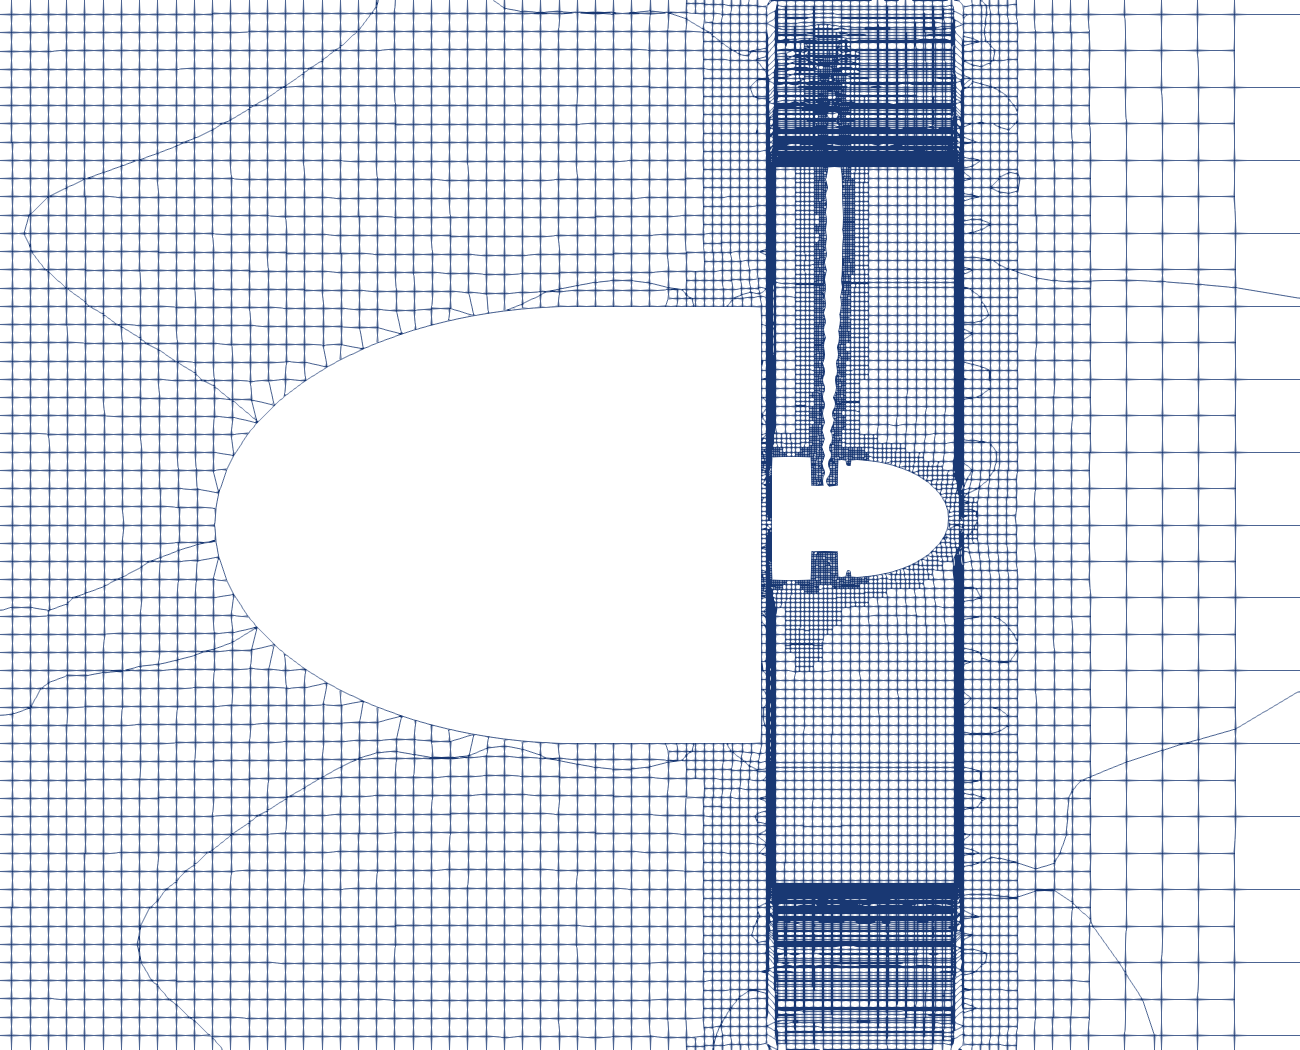
\includegraphics[height=5.2cm]{flow_7_maillage_coupe.png}\hfill
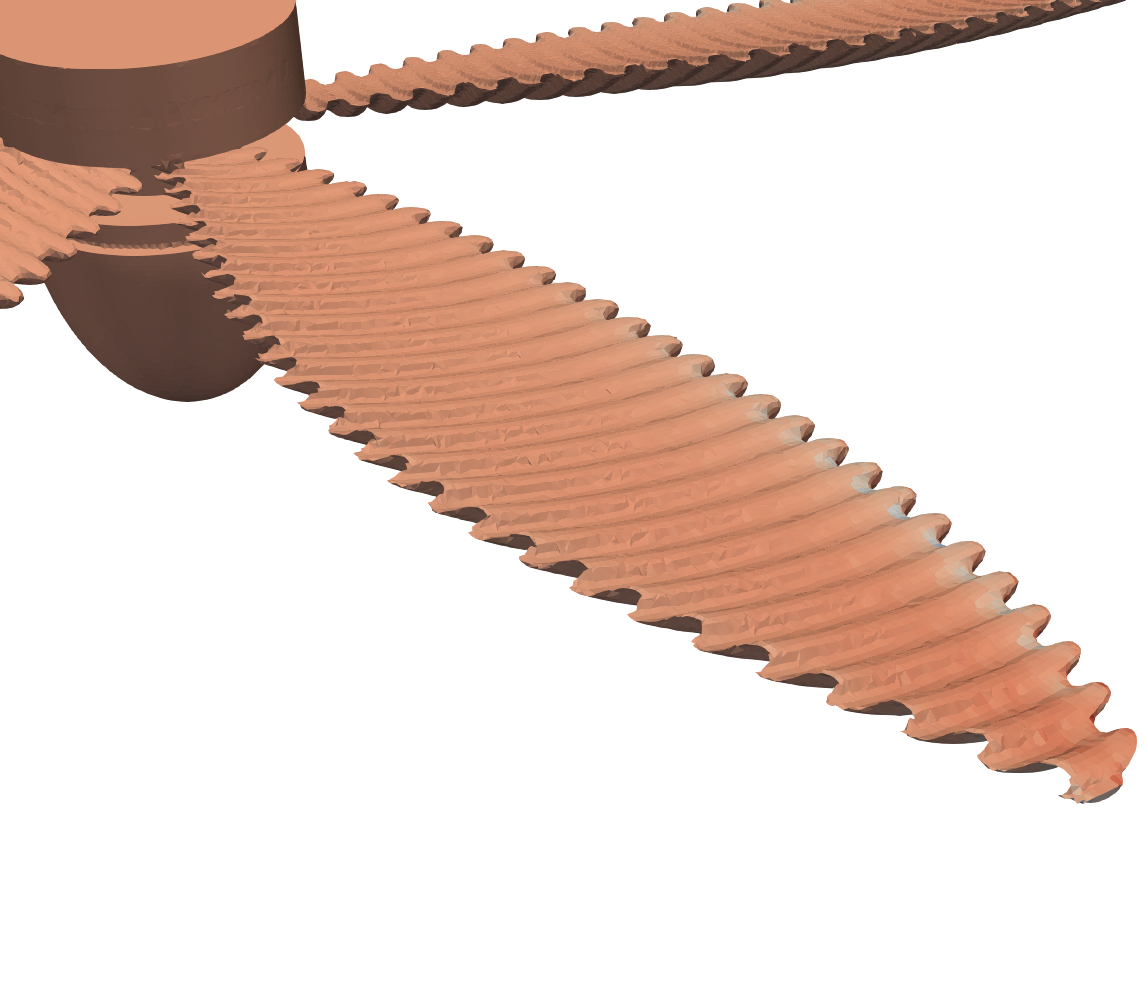
\includegraphics[height=5.2cm]{serrations_closeup.png}
\caption{Left: meridional cut of the mesh, from the far field to the blade band and the AMI cylinder
($R=\SI{72}{mm}$). Right: serrated trailing edges as resolved by the mesh.}
\label{fig:mesh}
\end{figure}

\begin{table}[h]
\centering
\caption{\texttt{checkMesh} on the retained mesh (June 2026 report).}
\label{tab:checkmesh}
\begin{tabular}{lr}
\toprule
Cells / points & \num{1949584} / \num{2205401} \\
Max aspect ratio & 6.61 \\
Max / mean non-orthogonality & 61.4 / 8.2 \\
Max skewness & 7.25 (12 faces above 4) \\
Concave cells & \num{49827} (2.6\,\%) \\
Cells with determinant $<0.001$ & 1851 \\
AMI weights (min / mean / max) & 0.90 / 1.002 / 1.27 \\
\bottomrule
\end{tabular}
\end{table}

\subsection{Solver, time strategy and computing}

\texttt{pimpleFoam} is run with three outer correctors, two pressure correctors and one non-orthogonal corrector.
Momentum convection uses \texttt{linearUpwindV}, $k$ and $\omega$ use \texttt{limitedLinear}, and time integration is
first-order implicit Euler. Phase~1, from rest to \SI{0.19}{s} (4.8 revolutions), uses an adaptive time step with a
Courant limit of 3 and $\Delta t\le\SI{1e-4}{s}$. Phase~2 restarts with a fixed $\Delta t=\SI{3.5e-5}{s}$
(227 steps per BPF period) and the FW-H function object, up to \SI{0.39}{s}; the fixed step is confirmed by the force
output, written every 10 steps at a uniform \SI{3.5e-4}{s}. The FW-H pressure is sampled every 5 steps
($f_s=\SI{5714}{Hz}$) in two records of \SI{100}{ms}. The solver runs only with floating-point trapping off
(\texttt{FOAM\_SIGFPE=false}) because of the degenerate cells.

Stable transient runs required three changes. A first attempt with the non-conformal coupling of OpenFOAM.org stopped
in the mesh stitcher after about \SI{200}{\micro s} on six mesh variants, so the case moved to cyclicAMI on the ESI
release; \texttt{snappyHexMesh} has to run in serial, because the parallel run aborted while load-balancing the AMI
faceZone; and the pressure solver was switched from GAMG to PCG on the coarse test mesh. The runs used a two-node
Linux cluster built for this project (8 and 4 cores, MPI over Ethernet); one node saturates at 4 cores, and
splitting the AMI case across both nodes gave no gain, so the nodes ran independent cases.

\subsection{Acoustic post-processing}\label{sec:post}

Each FW-H record begins with a start-up transient (on the axial microphones its peak reaches 35 to 52 robust
standard deviations of the rest of the record). The first \SI{15}{ms} of each record are discarded, which leaves two
segments of \SI{85}{ms} (486 samples) separated by a \SI{15}{ms} gap. Each segment has its mean and linear trend
removed, is Hann-windowed and zero-padded to 8192 points, and the two power spectra are averaged; the true
resolution is \SI{11.8}{Hz}. Tone levels are the peaks within $\pm\SI{6}{Hz}$ of $n$ and of the BPF, and the local
floor is the median level between 140 and \SI{240}{Hz}. Appendix~\ref{app:audit} explains why the segments are not
concatenated and no filter is applied.

\section{Verification}\label{sec:verif}

\paragraph{Established regime.} The force record available here starts at a restart at \SI{0.151}{s}
(Figure~\ref{fig:loads}). Averaged over successive revolutions, the thrust changes by \SI{1.9}{\%} between the
revolutions starting at 3.8 and 4.8 rotor turns, and by \SI{0.7}{\%} between 4.8 and 5.8 turns.

\begin{figure}[h]
\centering
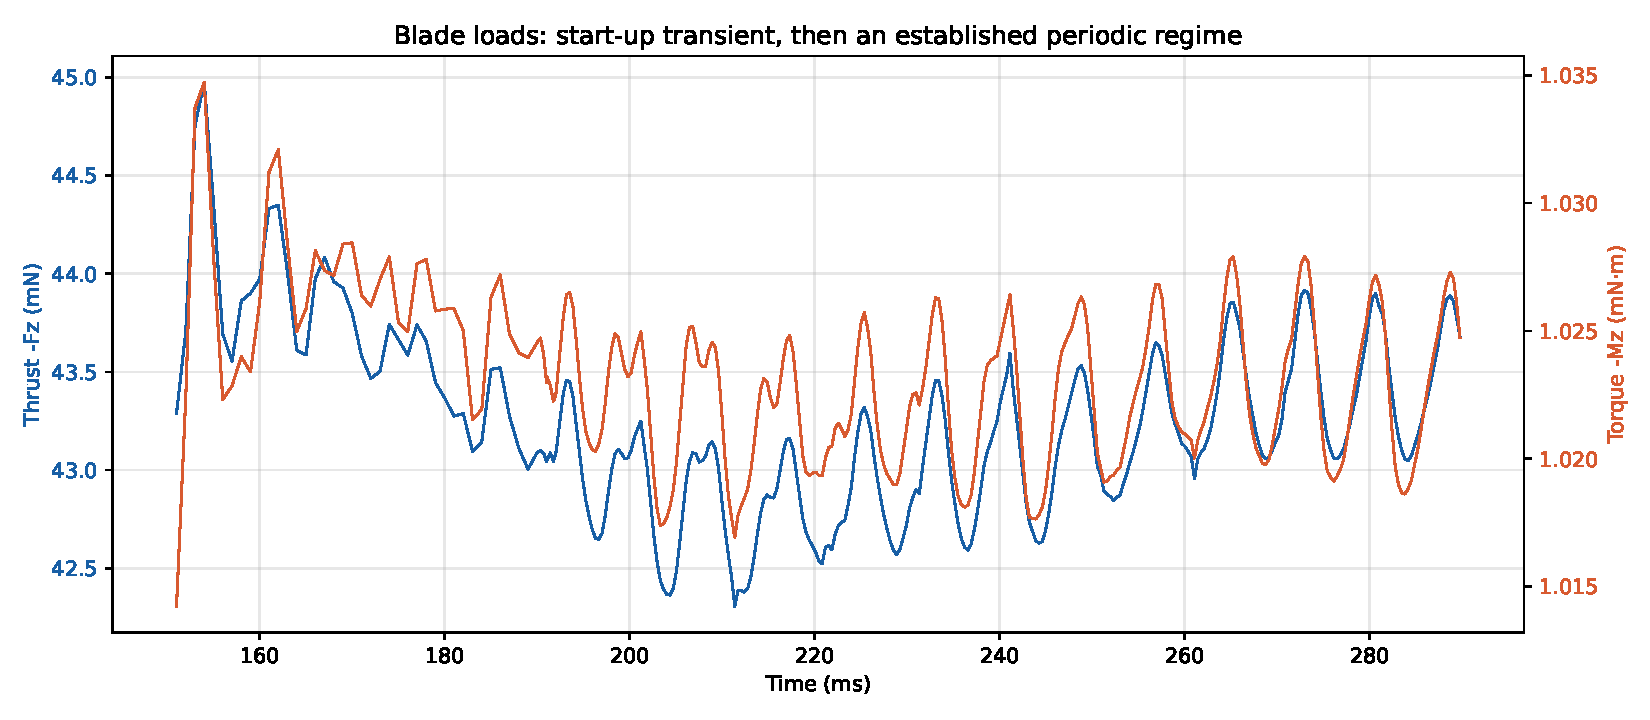
\includegraphics[width=0.82\linewidth]{blade_loads_time.pdf}
\caption{Thrust and torque on the blades from the restart at \SI{0.151}{s}: the jump at the restart, then a periodic
regime.}
\label{fig:loads}
\end{figure}

\paragraph{Coherence between records.} On the radial and $45^\circ$ microphones, a sine fit at \SI{25.15}{Hz} on the
absolute time axis gives the same level and the same phase ($148^\circ$) in both segments. On the axial microphones
the fitted phase changes between segments and the level stays at the floor.

\paragraph{Force-based check of the FW-H amplitudes.} At \SI{0}{Hz}, \SI{25}{Hz} (wavelength \SI{13.6}{m}) and the
BPF (\SI{2.7}{m}) the rotor is compact, so its loading noise reduces to that of the net force on the blades applied at
the hub \citep{lowson1965}:
\begin{equation}
  p'(\mathbf{x},t)=\frac{1}{4\pi}\left[\frac{x_i}{c_0r^2}\frac{\mathrm{d}F_i}{\mathrm{d}t}+\frac{x_iF_i}{r^3}\right]_{t-r/c_0},
  \qquad |p'|=\frac{A}{4\pi r}\sqrt{\left(\frac{\omega}{c_0}\right)^2+\frac{1}{r^2}}
  \label{eq:dipole}
\end{equation}
for a harmonic component of amplitude $A$ along the observer direction (the near-field term dominates at \SI{25}{Hz},
where $kr=0.46$). Because the FW-H surface integrates the blade pressure only, $F$ is the pressure part of the force
output. Table~\ref{tab:dipole} compares the estimates with the FW-H output over the same time window. The
directivities agree: the mean signal is $+1.24$, $-1.11$, $+0.86$ and \SI{\approx0}{mPa} on the downstream, upstream,
$45^\circ$ and radial microphones, the $\cos\theta$ pattern of the axial force, and the \SI{25}{Hz} tone is absent on
the axis and \SI{3.1}{dB} weaker at $45^\circ$ than in the plane ($\cos 45^\circ$ gives \SI{3.0}{dB}). The amplitudes do
not. The steady case is the simplest: it involves no time derivative and no retardation, yet the FW-H mean is 0.35
times the estimate. On the axis $M_r=0$ and $\dot{\mathbf{n}}\cdot\hat{\mathbf{z}}=0$ for a rotation about $z$, so
the FW-H integrand there is that of a fixed surface, and the surface motion cannot explain the axial gaps. The first
suspect is the input to the acoustic step (pressure scaling, surface normals, or the library output convention); it
has not been tested.

\begin{table}[h]
\centering
\caption{FW-H output against the compact-dipole estimate (\ref{eq:dipole}) from the blade pressure force
($r=\SI{1}{m}$; script \texttt{paper/scripts/dipole\_check.py}).}
\label{tab:dipole}
\small
\begin{tabular}{lrrr}
\toprule
Tone, microphone & force amplitude (mN) & compact dipole (dB) & FW-H (dB) \\
\midrule
25 Hz, radial (+x) & 0.94 & 9.3 & 21.2 \\
25 Hz, axis & -- & no radiation & at floor \\
BPF (124.5 Hz), downstream axis & 0.36 & 8.1 & -9.8 \\
\bottomrule
\end{tabular}

\end{table}

\paragraph{Not verified.} No mesh-independence study (one mesh), no second time step, no resolved boundary layer on
the blades, the phase-2 Courant number is not available (its log is on the offline cluster), and nothing is compared
with a measurement.

\section{Results}

\subsection{Aerodynamics}

Averaged over the last \SI{50}{ms} of the force record, the rotor gives \SI{43.3}{mN} of thrust and \SI{1.023}{mN.m}
of torque, that is an aerodynamic power $C\Omega=\SI{0.162}{W}$. The flow rate through a cut \SI{60}{mm} downstream of
the rotor is \SI{30.1}{L/s} (\SI{108}{m^3/h}). The blades drive an annular jet along the duct wall, with a slow
recirculating wake behind the hub (Figure~\ref{fig:flow}).

\begin{figure}[h]
\centering
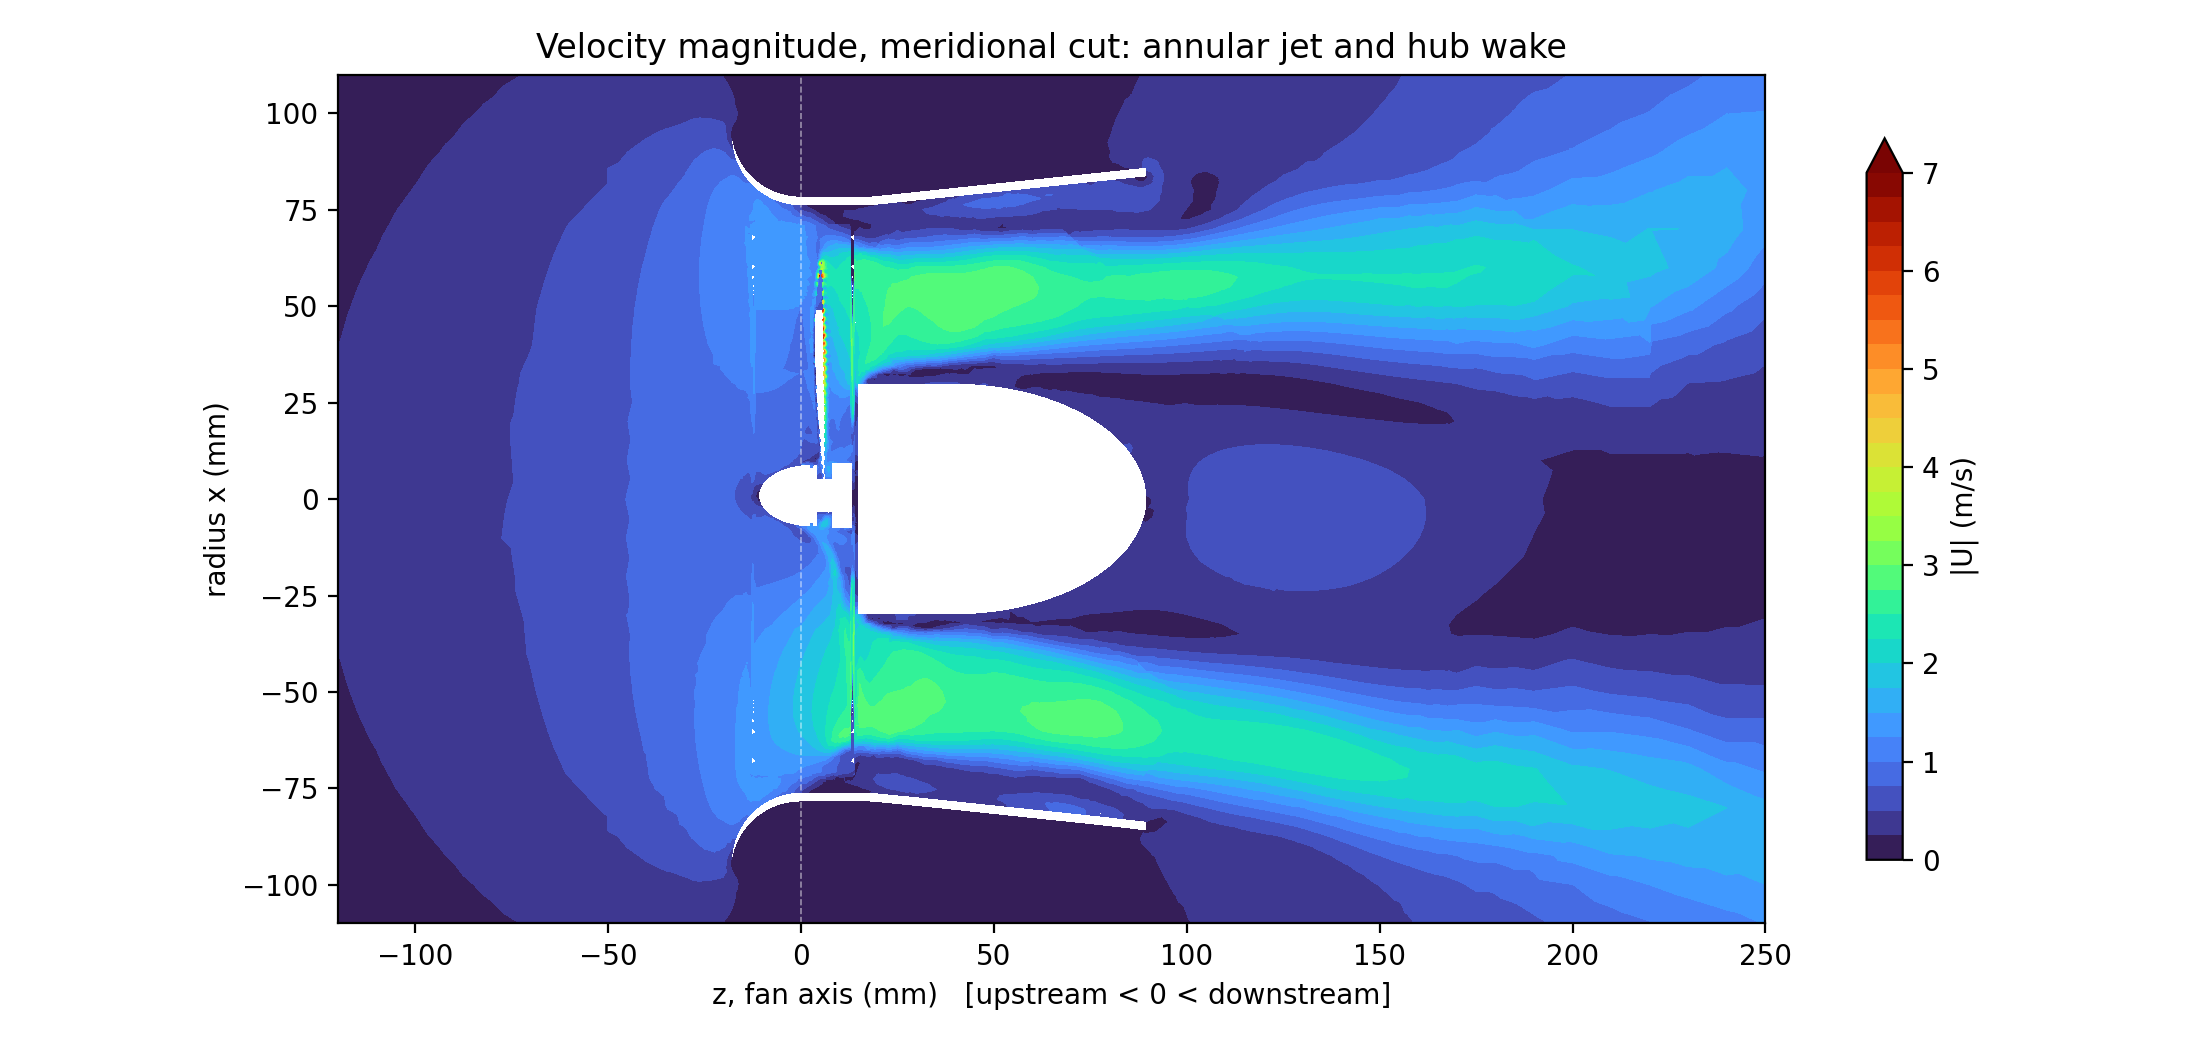
\includegraphics[width=0.88\linewidth]{meridional_velocity.png}
\caption{Velocity magnitude in the meridional plane at the last time step.}
\label{fig:flow}
\end{figure}

\subsection{Spectra}

Figure~\ref{fig:spl} shows the averaged spectra relative to each microphone's floor, and Table~\ref{tab:tones} the
tone levels. The BPF stands 20 to \SI{28}{dB} above the floor on all four microphones; its second harmonic appears on
every microphone and its third on all but the radial one. The once-per-revolution tone dominates in the rotor plane
and is absent on the axis. Neither tone should reach the axis from a perfectly symmetric rotor: a steady rotating
loading of five identical blades radiates only modes $m=5k$, and rotor--arm interaction with three arms gives
$m=5k-3s$, so the axisymmetric mode $m=0$ that radiates on the axis first appears at $3\times$BPF \citep{tyler1962}.
The on-axis BPF, like the \SI{25}{Hz} tone, therefore implies a loss of five-fold symmetry in the computed loading.

\begin{figure}[h]
\centering
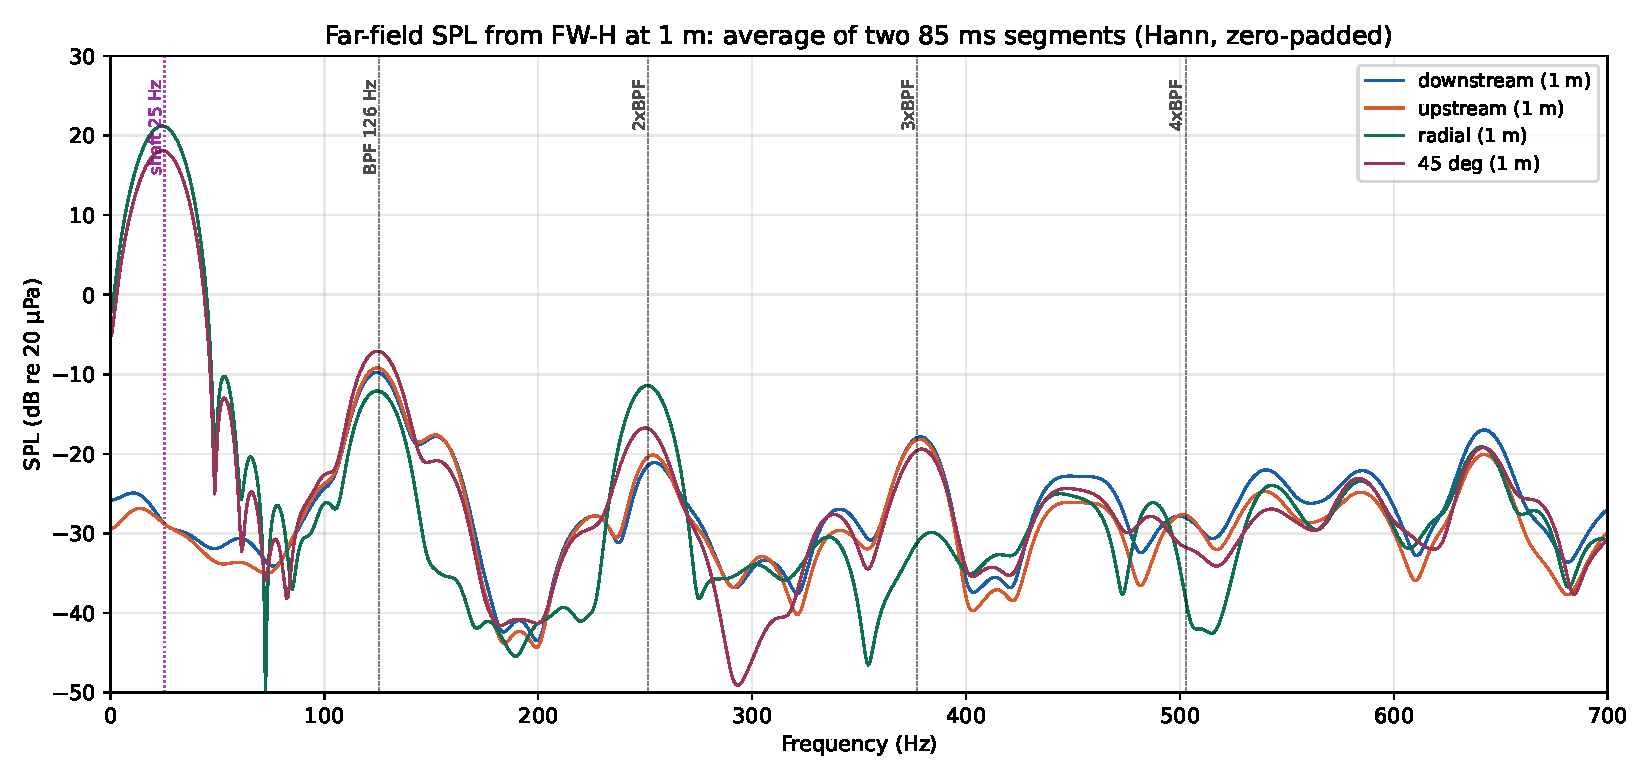
\includegraphics[width=\linewidth]{spl_spectrum.pdf}
\caption{FW-H spectra at \SI{1}{m} relative to each microphone's floor (140--\SI{240}{Hz}): average of the two
\SI{85}{ms} segments, Hann window, raw signal. Shaded: the line comb of Section~\ref{sec:comb}.}
\label{fig:spl}
\end{figure}

\begin{table}[h]
\centering
\caption{Tone levels at \SI{1}{m} (dB re \SI{20}{\micro Pa}, raw signal). Absolute levels are not reliable
(Section~\ref{sec:verif}); only comparisons between microphones and tone-to-floor ratios are used.}
\label{tab:tones}
\begin{tabular}{lrrrr}
\toprule
Microphone & \SI{25}{Hz} & BPF & floor (140--\SI{240}{Hz}) & BPF $-$ floor \\
\midrule
Downstream (axis) & $-26.7$ (floor) & $-9.8$ & $-30.0$ & 20.3 \\
Upstream (axis) & $-27.5$ (floor) & $-9.2$ & $-30.1$ & 20.9 \\
Radial & 21.2 & $-12.1$ & $-39.8$ & 27.7 \\
$45^\circ$ downstream & 18.1 & $-7.1$ & $-30.1$ & 23.0 \\
\bottomrule
\end{tabular}
\end{table}

\subsection{Once-per-revolution tone}

The net pressure force on the blades has an in-plane component of \SI{0.77}{mN} that rotates with the rotor: $F_x$
and $F_y$ oscillate at \SI{25.15}{Hz} with equal amplitudes. As shown in Section~\ref{sec:verif}, the \SI{25}{Hz}
directivity is that of this rotating force. Whether the imbalance comes from the STL and mesh (the surfaces are
faceted) or from the flow was not established.

\subsection{High-frequency line comb}\label{sec:comb}

Above \SI{600}{Hz} the spectra contain lines at 642, 742, 843, 943, 1044, 1144, 1244, 1346 and \SI{1446}{Hz}, spaced
\SI{100.5}{Hz}, up to \SI{44}{dB} above the floor on the radial microphone; on the axial microphones they carry about
90\,\% of the signal variance. The lines continue up to \SI{2}{kHz}. They come from bursts in the axial blade force that
reach the FW-H signal about \SI{3}{ms} later, the propagation time over \SI{1}{m} (Figure~\ref{fig:comb}). A
straight-line fit of the ten burst centres gives a period of $9.943\pm\SI{0.011}{ms}$: a quarter revolution
(\SI{9.944}{ms}), and five standard errors away from the \SI{10}{ms} field write interval. The bursts are locked to
the rotor, four times per revolution. No physical source with that order is expected for five blades and three arms;
the probable cause is the four-fold symmetry of the box and of the Cartesian background mesh seen by the rotor through
the AMI interface. The comb is treated as numerical and lies above the tones studied here.

\begin{figure}[h]
\centering
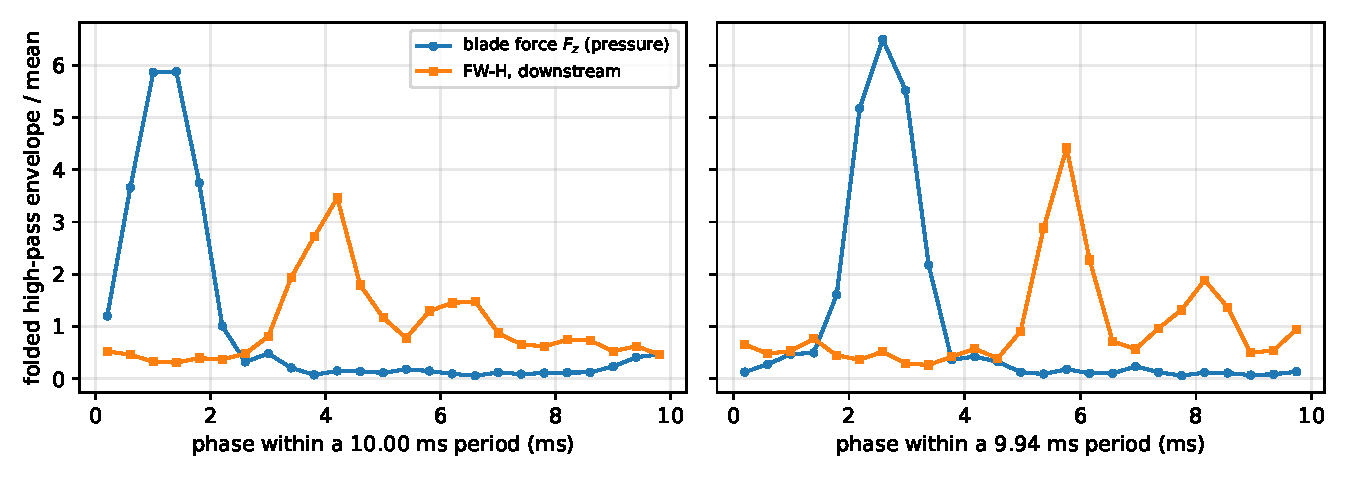
\includegraphics[width=0.9\linewidth]{comb_fold.pdf}
\caption{Envelope of the high-passed ($>\SI{600}{Hz}$) axial blade force and downstream FW-H signal, folded on
\SI{10.00}{ms} (left, field write interval) and \SI{9.94}{ms} (right, a quarter revolution); the fold is sharper on the right. Script \texttt{paper/scripts/comb\_check.py}.}
\label{fig:comb}
\end{figure}

\section{Discussion and limitations}

The flow shows the expected annular jet. In the acoustic output, the frequencies and directivities are consistent with
the blade forces, while the amplitudes are not; the on-axis BPF and the \SI{25}{Hz} tone both imply a loss of
five-fold symmetry, and the line comb above \SI{600}{Hz}, locked to the rotor four times per revolution, is probably numerical. The limits are:
\begin{itemize}
  \item \emph{Amplitudes.} The FW-H levels differ from the force-based estimates by $-18$ to $+14$~dB
    (Table~\ref{tab:dipole}).
  \item \emph{Resolution.} Two \SI{85}{ms} segments give \SI{11.8}{Hz}. A contiguous \SI{0.4}{s} record would take
    more than \SI{100}{h} on the 1.95 M-cell mesh (the measured cost is \SI{16.5}{s} per step on the 0.91 M-cell mesh),
    and the cluster holding the restart data was offline in October 2026.
  \item \emph{Numerical accuracy.} One mesh, one time step, first-order time integration (227 steps per BPF period in
    phase 2), no prism layers, \num{49827} concave cells, and solver runs with floating-point trapping off.
  \item \emph{Domain.} The lateral boundaries are \SI{0.2}{m} from the axis, 2.6 duct radii; their effect on the jet
    and on the rotor loading was not tested.
  \item \emph{Physics.} URANS resolves tonal noise only. Serrations act mainly on broadband noise
    \citep{howe1991,lyu2016}, and no smooth-blade reference was run, so this study does not measure their effect. The
    FW-H surface covers the blades only.
  \item \emph{No measurement.} Thrust, flow rate and spectra are not compared with tests.
\end{itemize}

\section{Conclusion and future work}

A sliding-mesh URANS and FW-H chain gives \SI{43.3}{mN} of thrust and \SI{108}{m^3/h} at \SI{1509}{rpm} for the
serrated ducted fan, with a BPF tone and harmonics on all microphones and a once-per-revolution tone confined to the
rotor plane. Checking the FW-H output against the integrated blade force agreed on its directivities and showed that
its amplitudes are not reliable. In order of priority: run the acoustic step on a case with a known answer (a
stationary or rotating compact dipole) to locate the amplitude error; test the line comb with a rotated or cylindrical background
mesh; record a contiguous signal of at least \SI{0.4}{s}; add two meshes and a second time step; and run
a smooth-blade reference rotor before drawing any conclusion on the serrations.

\section*{Reproducibility statement}

Case files: \path{openfoam_case/} (phase~1 \path{system/controlDict}, phase~2 \path{system/controlDict.phase2}, mesh
\path{system/snappyHexMeshDict}); the STL geometry is not published. The published records were computed on the
cluster with OpenFOAM v2506 and libAcoustics; the earlier 0.91 M-cell run used OpenFOAM v2406 under WSL. From the
repository root (Python 3, numpy, scipy, matplotlib; seconds per script):
\path{postprocessing/acoustics/post_acoustique_combine.py} (Table~\ref{tab:tones}, Figures~\ref{fig:spl} and
\ref{fig:audit}), \path{postprocessing/aero/perf_aero.py} (thrust, torque, power, Figure~\ref{fig:loads}),
\path{paper/scripts/dipole_check.py} (Table~\ref{tab:dipole}), \path{paper/scripts/comb_check.py}
(Figure~\ref{fig:comb}). The flow rate and Figure~\ref{fig:flow} need ParaView slices that are not published
(\path{postprocessing/rendering/render_flow_2d.py}). The paper is rebuilt with \path{paper/build_paper.sh}.

\bibliographystyle{unsrtnat}
\bibliography{references}

\appendix
\section{Audit of the first acoustic analysis}\label{app:audit}

The first analysis of these records concatenated the two segments and applied a 5-point median filter against
numerical spikes. The concatenation joins segments \SI{15}{ms} apart, which puts a phase jump of
$360^\circ\times\SI{15}{ms}\times\SI{25.15}{Hz}\approx136^\circ$ into the once-per-revolution component and splits its
peak. The segments contain few outlier samples (at most 4 beyond 5 robust standard deviations), and the filter raises
the floor by 9 to \SI{24}{dB}, hides the BPF harmonics and moves the radial BPF level by about \SI{4}{dB}
(Figure~\ref{fig:audit}). Both steps were dropped.

\begin{figure}[h]
\centering
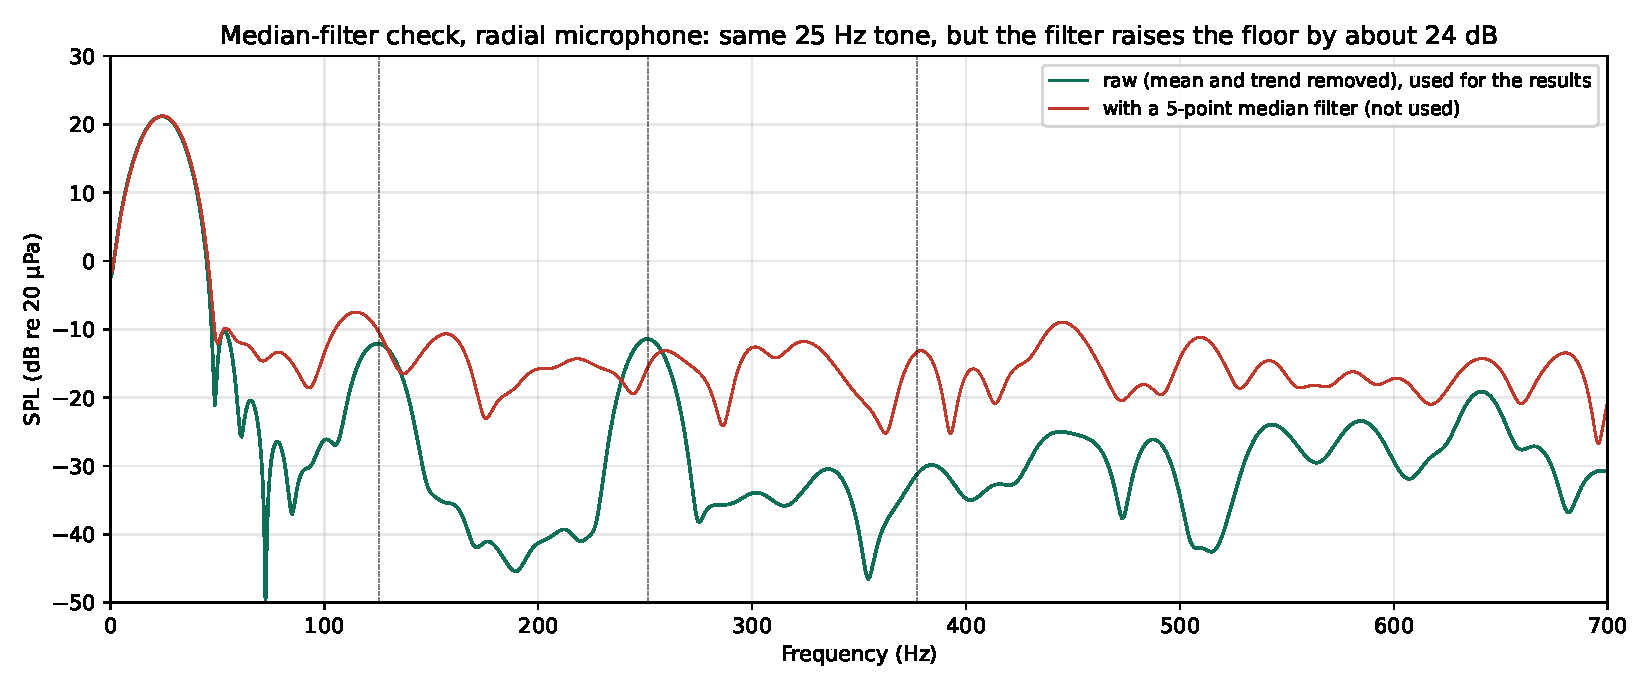
\includegraphics[width=0.85\linewidth]{raw_vs_filtered.pdf}
\caption{Radial microphone, average of the two segments: raw signal (used) and 5-point median filter (not used).}
\label{fig:audit}
\end{figure}

\end{document}
